\documentclass[9pt]{beamer}
\usepackage{kotex}
\usepackage{amsfonts,amssymb,amsthm}
\usepackage[dvipsnames]{xcolor}
\usepackage{xcolor}
\usepackage{etoolbox}
\usepackage{braket}
\usepackage{qcircuit}

%## color
\definecolor{customBlack}{HTML}{3B4252}
\definecolor{customBlackGrey}{HTML}{434C5e}
\definecolor{cuatomGrey}{HTML}{4C566A} 
\definecolor{customWhite}{HTML}{ECEFF4} 
\definecolor{customBlue}{HTML}{6082B6}  
\definecolor{customRed}{HTML}{BF616A}
\definecolor{vividauburn}{rgb}{0.58, 0.15, 0.14}


%## Theme & custom
% \usetheme{metropolis}           % Use metropolis theme
% \metroset{block=fill}
\usetheme{moloch} % modern fork of the metropolis theme
\molochset{block=fill}
\setbeamersize{text margin left=5mm, text margin right=5mm}
\setbeamercolor{palette primary}{bg=customBlack}
\setbeamercolor{alerted text}{fg=customRed}
\setbeamercolor{itemize item}{fg=customBlue}
\setbeamercolor{enumerate item}{fg=customBlue}


%## font
\usefonttheme[onlymath]{serif}
% \setbeamerfont{normal text}{size=\small}
% \setbeamerfont{math text}{size=\tiny}


%## Theorem title, numbering
\makeatletter
\setbeamertemplate{theorem begin}
{%
\begin{\inserttheoremblockenv}
{%
\inserttheoremheadfont
\inserttheoremname
\ifx\inserttheoremaddition\@empty\else\ of\ \inserttheoremaddition\fi%
\inserttheorempunctuation
}%
}
\setbeamertemplate{theorem end}{\end{\inserttheoremblockenv}}
\makeatother
\setbeamertemplate{theorems}[numbered]  


%## Custom block
\setbeamercolor{block title}{bg=customBlue, fg=white}
\setbeamercolor{block body}{bg=customWhite, fg=customBlack}
\setbeamercolor{block title alerted}{%
    use={block title, alerted text},
    bg=customRed,
    fg=white
}
\setbeamercolor{block body alerted}{%
    use={block title, alerted text},
    bg=customWhite,
    fg=customBlack
}
\AtBeginEnvironment{definition}{%
    \setbeamercolor{block title}{fg=white,bg=customBlackGrey}
    \setbeamercolor{block body}{fg=customBlack, bg=customWhite}
}
\AtBeginEnvironment{theorem}{%
    \setbeamercolor{block title}{fg=white,bg=customBlackGrey}
    \setbeamercolor{block body}{fg=customBlack, bg=customWhite}
}
\AtBeginEnvironment{corollary}{%
    \setbeamercolor{block title}{fg=white,bg=customBlackGrey}
    \setbeamercolor{block body}{fg=customBlack, bg=customWhite}
}
\AtBeginEnvironment{lemma}{%
    \setbeamercolor{block title}{fg=white,bg=customBlackGrey}
    \setbeamercolor{block body}{fg=customBlack, bg=customWhite}
}


%! Useful command
\renewcommand{\Pr}{\text{Pr}}
% $\ast$ \underline{Proof}:
%\checkmark \underline{meaning}:

\title{5. Quantum Algorithm}
\date{\today}
\author{Vaughan Sohn}
% \institute{Centre for Modern Beamer Themes}


\begin{document}
    %#################################### 
    \maketitle
    
    %#################################### 
    \begin{frame}
        \frametitle{Contents}
        \tableofcontents
    \end{frame}
    
    %#################################### 
    \begin{section}{Deutsch's Algorithm}
        \begin{frame}
            \frametitle{Design Quantum Algorithm}
            \begin{itemize}
                \item Algorithm은 어떤 문제를 해결하는 동안, 다양한 \textit{function}을 호출할 수 있다.
                \item 따라서 Quantum Algorithm을 설계하기 위해서는 어떤 주어진 \textit{function}을 quantum computer에서 나타낼 수 있는 방법이 필요하다.
            \end{itemize}
            \vspace{0.3cm}
            \textbf{Represent boolean function}
            \\ 다음 boolean function을 unitary gate $U_f$로 구현해보자.
            $$ f: \{0, 1\} \rightarrow \{0, 1\} $$ 
            \vspace{-0.2cm}
            \begin{itemize}
                \item one-qubit gate: 
                \\\textit{Problem}: $f$가 constant, 즉 non-invertable이라면 unitary가 아니다.
                $$ \ket x \rightarrow \ket{f(x)} $$
                \item \underline{two-qubit} gate:
                \begin{itemize}
                    \item ancilla qubit을 추가하여 two-qubit gate로 설계하면 unitary 조건을 만족한다.
                    \item $\ket q$를 $\ket 0$으로 설정하면 연산 결과, $\ket q$가 $f(x)$가 된다.
                \end{itemize}
                $$\ket x \ket q \rightarrow \ket x \ket{q \oplus f(x)}$$
            \end{itemize}
        \end{frame}

        \begin{frame}
            \frametitle{Design Quantum Algorithm}
            \textbf{Advantage of Quantum Algorithm}
            
            \begin{itemize}
                \item Unitary gate $U_f$의 입력을 \textit{superposition state} $\ket x = \ket +$로 설정하게 되면, 단 한번 unitary gate를 통과함으로서 모든 input $0, 1$에 대한 결과를 얻을 수 있다.
                $$\ket + \ket 0 \rightarrow \frac{1}{\sqrt{2}} \left( \ket 0 \ket{f(0)} + \ket 1 \ket{f(1)} \right) $$
                \item \textit{More generally}, $f: \{0, 1\}^n \rightarrow \{0, 1\}$에 대한 unitary에 superposition state를 제공하면 다음 상태를 얻는다.
                $$\ket +^{\otimes n} \ket 0 \rightarrow \frac{1}{\sqrt{2^n}}\sum_{x \in \{0, 1\}^n} \ket x \ket{f(x)}$$
            \end{itemize}
            
        \end{frame}

        \begin{frame}
            \frametitle{Deutsch's Problem}
            \underline{Problem}: 주어진 one-bi function $f: \{0, 1\} \rightarrow \{0, 1\}$이 constant인지 balance인지를 판단하는 문제
            \vspace{0.2cm}
            \begin{itemize}
                \item 가능한 4가지 함수 중에서 constant / balance function은 각각 다음과 같이 구분된다.
                \item $f(0) \oplus f(1)$의 값을 구할 수 있다면, 함수가 constant인지 아닌지를 구분할 수 있다.
                $$ \begin{cases} \text{constant} & \text{ if } f(0)\oplus f(1) = 0  \\ \text{balance} & \text{ if } f(0)\oplus f(1) = 1 \end{cases}$$
            \end{itemize}
            \begin{figure}
                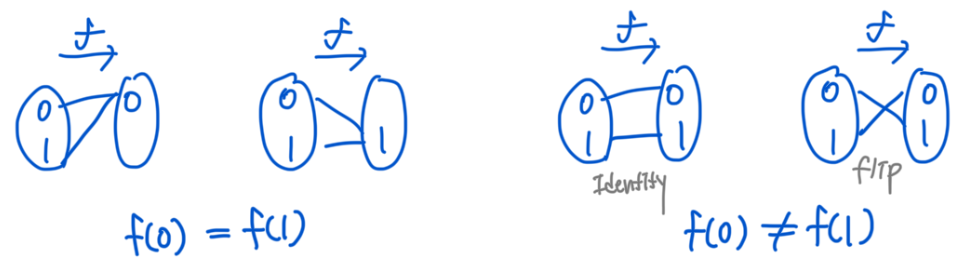
\includegraphics[width=0.6\textwidth]{image/L5_Deutsh.png}
            \end{figure}
        \end{frame}

        \begin{frame}
            \frametitle{Deutsch's Algorithm}
            \underline{Solutions}: 
            \vspace{0.2cm}
            \begin{itemize}
                \item classically, 주어진 함수 $f$에 대해 서로 다른 입력에 대해 \alert{2번} 호출하면 $f(0), f(1)$의 결과를 알 수 있으므로 constant인지 balance인지를 구분할 수 있다.
                \item quantumly, 다음과 같이 구성한 quantum circuit을 실행하면, $U_f$를 \alert{1번} 호출하는 것만으로 함수가 constant인지 balance인지를 구분할 수 있다. 
                \item $U_f$는 다음의 동작을 수행하는 unitary gate이다.
                $$U_f\ket x \ket y = \ket x \ket{y\oplus f(x)} $$
            \end{itemize}
            %? Deutsh
            \begin{table}[h]
                \[
                \begin{array}{c}
                \Qcircuit @C=1.1em @R=.8em {
                    \lstick{\ket{0}} &   \gate{H}   \barrier[-1.6em]{1}   & \multigate{1}{U_f}   \barrier[-1.3em]{1}   &  \gate{H}   \barrier[-1.4em]{1}   & \meter\\
                    \lstick{\ket{1}} &   \gate{H} & \ghost{U_f}          & \qw       & \meter
                }
                \end{array}
                \]
            \end{table}
        \end{frame}

        \begin{frame}
            \frametitle{Deutsch's Algorithm}
            앞에서 제안한 quantum circuit을 이용하면 정말로 문제를 해결할 수 있는지 확인해보자. 각각의 gate를 통과한 뒤 system의 state는 다음과 같이 변화하게 된다.
            \vspace{0.2cm}
            \begin{enumerate}
                \item $H \otimes H$
                \item $U_f$
                \vspace{1.3cm}
                \item $H \otimes I$
                \vspace{1.3cm}
            \end{enumerate}
            따라서 측정 전, 최종 상태는 다음과 같다.
            $$ (-1)^{f(0)} \frac{1}{2} \Big((\ket 0 + \ket 1) + (-1)^{f(0) \oplus f(1)}(\ket 0 - \ket 1)\Big) \ket - $$
        \end{frame}

        \begin{frame}
            \frametitle{Deutsch's Algorithm}
            Deutsch Algorithm에서 얻은 최종 상태는 다음과 같다.
            $$ (-1)^{f(0)} \frac{1}{2} \Big((\ket 0 + \ket 1) + (-1)^{f(0) \oplus f(1)}(\ket 0 - \ket 1)\Big) \ket - $$

            이 상태는 $f(0) \oplus f(1)$의 값이 $0$인지 $1$인지에 따라서 다음 둘 중 하나의 상태가 된다.
            $$= \begin{cases} (-1)^{f(0)}\ket 0 \ket - & \text { if } f(0)\oplus f(1)=0\ :const \\ (-1)^{f(0)}\ket 1 \ket - & \text { if } f(0)\oplus f(1)=1\ :balanced\end{cases}$$
            
            \vspace{0.5cm}
            $\Rightarrow$ 따라서 첫번째 qubit의 값을 측정하여 $f(0)\oplus f(1)$의 값을 알아낼 수 있다.$\Box$
            
            \vspace{0.4cm}

            \begin{alertblock}{Idea: global / relative phase}
                $f$가 constant 함수라면 global phase $(-1)^{f(0)}$만 가해지기 때문에 처음 상태와 동일한 상태가 된다. 하지만 $f$가 balanced 함수라면 relative phase $(-1)$이 가해지면서 qubit의 값이 $\ket 1$로 변화된다.
            \end{alertblock}
        \end{frame}


        \begin{frame}
            \frametitle{Deutsch's-Jozsa Algorithm}
            \underline{Problem}: 주어진 n-bit function $f: \{0, 1\}^n \rightarrow \{0, 1\}$이 constant인지 balance인지를 판단하는 문제
            \vspace{0.2cm}

            \underline{Solutions}: 
            \vspace{0.2cm}
            \begin{itemize}
                \item classically, 최악의 경우 $2^{n-1}+1$번 함수를 호출해야한다. ($O(2^n)$)
                \item quantumly, Deutsch's algorithm을 활용하면 $U_f$를 \alert{1번} 호출하는 것만으로 함수가 constant인지 balance인지를 구분할 수 있다. 
                \item $U_f$는 다음의 동작을 수행하는 unitary gate이다.
                $$U_f\ket x \ket y = \ket x \ket{y\oplus f(x)} $$
                \textit{where} $\ket x = \ket {x_1x_2 \cdots x_{n}}$
            \end{itemize}
            %? Deutsh
            \begin{table}[h]
                \[
                \begin{array}{c}
                \Qcircuit @C=1.1em @R=.8em {
                    \lstick{\ket{0}} & {/^{\otimes n} } \qw& \gate{H^{\otimes n}}   \barrier[-1.6em]{1}   & \multigate{1}{U_f}   \barrier[-1.9em]{1}   &  \gate{H^{\otimes n} }   \barrier[-1.4em]{1}   & \meter\\
                    \lstick{\ket{1}}  & \qw & \gate{H} & \ghost{U_f}          & \qw       & \meter
                }
                \end{array}
                \]
            \end{table}
        \end{frame}

        \begin{frame}
            \frametitle{Deutsch's-Jozsa Algorithm}
            앞에서 제안한 quantum circuit을 이용하면 정말로 문제를 해결할 수 있는지 확인해보자. 각각의 gate를 통과한 뒤 system의 state는 다음과 같이 변화하게 된다.
            \vspace{0.2cm}
            \begin{enumerate}
                \item $H^{\otimes n+1}$
                \item $U_f$
                \vspace{1.3cm}
                \item $H^{\otimes n} \otimes I$
                \vspace{1.3cm}
            \end{enumerate}
            따라서 측정 전, 최종 상태는 다음과 같다.
            $$\left(\sum_{z, x \in\{0,1\}^n} \frac{(-1)^{x \cdot z+f(x)}|z\rangle}{2^n}\right) \ket{-}.$$
            \vspace{-0.4cm}
        \end{frame}

        \begin{frame}
            \frametitle{Deutsch's-Jozsa Algorithm}
            주어진 $f(x)$가 constant function이라면,
            \begin{itemize}
                \item  $\forall x$에 대해서 $f(x)$의 결과는 항상 동일하기 때문에, 첫 번째 레지스터의 상태를 다음과 같이 표현할 수 있다. ($\ast$)
                $$ \frac{(-1)^{f(x)}}{2^n} \sum_{z, x \in\{0,1\}^n} {(-1)^{x \cdot z}|z\rangle}    $$
                \item 만약 $z = 0^n$이라면, $x \cdot z = 0^n$이 되어서 $\ket{0^n}$의 계수가 $\pm 1$이 된다.
                \item 따라서, 첫 번째 레지스터를 측정하면 100\%의 확률로 $\ket{0^{\otimes n}}$를 얻게된다.
            \end{itemize}
            \vspace{0.2cm}
            반면, $f(x)$가 balanced function이라면,
            \begin{itemize}
                \item 첫 번째 레지스터의 상태를 다음과 같이 표현할 수 있다.
                $$ \frac{1}{2^n} \sum_{z, x \in\{0,1\}^n} {(-1)^{f(x)}(-1)^{x \cdot z}|z\rangle}  $$
                \item 만약 $z = 0^n$이라면, $\ket{0^n}$의 계수는 $\Sigma (-1)^{f(x)}$에 의해 결정된다.
                \item $f$가 balance function이므로 $(-1)^{f(x)}$의 값이 정확히 반은 1, 반은 -1이 되기 때문에 이를 다 summation하게 되면 계수가 $0$이 된다.
                \item 따라서, 첫 번째 레지스터를 측정했을 때, $\ket{0^{\otimes n}}$을 얻을 확률은 0\%이다.$\Box$
            \end{itemize}
        \end{frame}
    \end{section}

    %#################################### 
    \begin{section}{Hamiltonian Simulation}
        \begin{frame}
            \frametitle{Hamiltonian Simulation Problem}
            
        \end{frame}

        \begin{frame}
            \frametitle{Hamiltonian Simulation by Trotter formular}
            
        \end{frame}

        \begin{frame}
            \frametitle{Error bound of Hamiltonian Simulation}
            
        \end{frame}
    \end{section}

    %#################################### 
    \begin{section}{Quantum Fourier Transformation}
        \begin{frame}
            \frametitle{Classical and Quantum Fourier Transform}
            
        \end{frame}

        \begin{frame}
            \frametitle{Implement Quantum Fourier Transform}
            
        \end{frame}
    \end{section}


    %#################################### 
    \begin{section}{Phase Estimation}
        \begin{frame}
            \frametitle{Phase estimation}
            
        \end{frame}

        \begin{frame}
            \frametitle{Error bound of Phase estimation}
            
        \end{frame}
    \end{section}
    \begin{frame}{References}
        
        \begin{itemize}
            \item M. A. Nielson and I. L. Chuang, Quantum Computation and Quantum Information
            \item Lecture notes for QU511: Quantum Computing (Fall 2024)
        \end{itemize}
        \vspace{6cm}
    \end{frame}


\end{document}